% vim: set textwidth=78 autoindent:
    
\subsection{Usar el complemento de texto delimitado}\label{label_dltext}    

El complemento de texto delimitado le permite cargar un archivo de texto delimitado 
como una capa en QGIS.
    
\subsubsection{Requisitos}

Para ver un archivo de texto delimitado como una capa, el archivo de texto debe contener:

\begin{enumerate}      
\item Una fila de encabezado delimitado con los nombres de los campos. Debe ser la primera 
línea del archivo de texto.
\item La fila de encabezado debe contener un campo X e Y. Estos campos se pueden llamar de 
cualquier forma.
\item Las coordenadas X e Y deben estar especificadas como números. El sistema de coordenadas 
no es importante.
\end{enumerate}

Un ejemplo de un archivo de texto válido tendría este aspecto:

\begin{verbatim} 
nombre|latdec|longdec|celda|
196 mile creek|61.89806|-150.0775|tyonek d-1 ne|
197 1/2 mile creek|61.89472|-150.09972|tyonek d-1 ne|
a b mountain|59.52889|-135.28333|skagway c-1 sw|
apw dam number 2|60.53|-145.75167|cordova c-5 sw|
apw reservoir|60.53167|-145.75333|cordova c-5 sw|
apw reservoir|60.53|-145.75167|cordova c-5 sw|
aaron creek|56.37861|-131.96556|bradfield canal b-6|
aaron island|58.43778|-134.81944|juneau b-3 ne|
aats bay|55.905|-134.24639|craig d-7|
\end{verbatim}


Algunos elementos a tener en cuenta  sobre los archivos de texto son:

\begin{enumerate}        
\item  El archivo de texto de ejemplo usa \mbox{$|$} como delimitador. Se puede usar 
cualquier carácter para delimitar los campos.
\item La primera fila es la fila de encabezado. Contiene los campos nombre, latdec,
longdec y celda.
\item No se usan comillas ({\tt{}"{}}) para delimitar campos de texto.
\item Las coordenadas X están en el campo {\em longdec}.
\item Las coordenadas Y están en el campo  {\em latdec}.
\end{enumerate}

\subsubsection{Usar el complemento}
Para usar el complemento debe estar ejecutando QGIS y usar el Administrador de 
complementos para cargarlo:

Inicie QGIS y abra el Administrador de complementos seleccionando el menú {\em
Complementos\mbox{$|$}Administrador de complementos}. El Administrador de complementos 
muestra una lista de todos los complementos disponibles. Aquellos que se encuentren ya 
cargados tendrán una marca a la izquierda del nombre. Marque la casilla que hay a la 
izquierda del complemento {\em Añadir capa de texto delimitado} y pulse Aceptar para 
cargarlo como se describe en la Sección \ref{sec:managing_plugins}.


Ahora habrá un nuevo icono en la barra de herramientas:
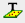
\includegraphics[width=0.7cm]{toolbar_icon}
Pulse el icono para abrir el diálogo de texto delimitado, tal como aparece en la Figura
\ref{fig:delim_text_plugin_dialog}.

\begin{figure}[ht]
   \begin{center}
   \caption{Diálogo de texto delimitado}\label{fig:delim_text_plugin_dialog}\smallskip
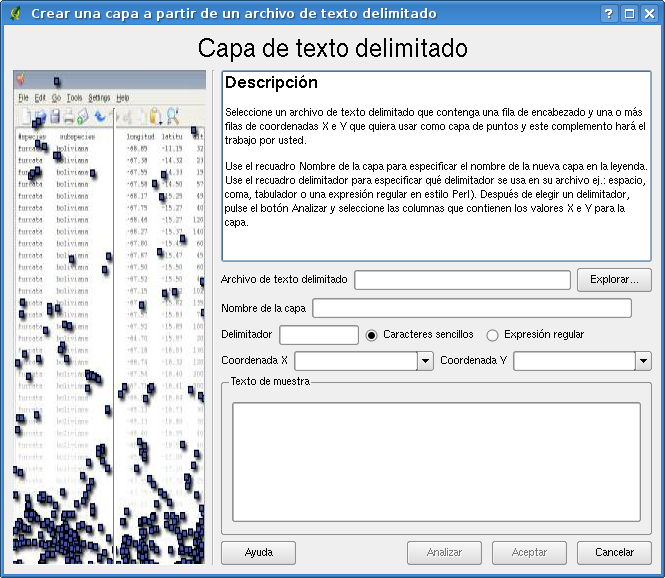
\includegraphics[clip=true, width=10cm]{dialog}
   \end{center}  
\end{figure}

Primero seleccione el archivo a importar pulsando en el botón \textit{Explorar...}.
Seleccione el archivo de texto deseado en el diálogo de archivos. Una vez seleccionado, 
el complemento intenta analizar el archivo usando el último delimitador empleado, en 
este caso \mbox{$|$} (vea la Figura \ref{fig:delim_text_file_selected}).

\begin{figure}[ht]
   \begin{center}
   \caption{Archivo seleccionado}\label{fig:delim_text_file_selected}\smallskip
\includegraphics[clip=true, width=10cm]{file_selected}   
   \end{center}  
\end{figure}
  
En este caso el delimitador \mbox{$|$} no es correcto para el archivo, que en
realidad está delimitado con tabulador. Vea que los campos desplegables X e Y
no contienen nombre de campo válidos.

\begin{figure}[ht]
   \begin{center}
   \caption{Campos analizados del archivo de texto}\label{fig:delim_text_file_selected2}\smallskip  
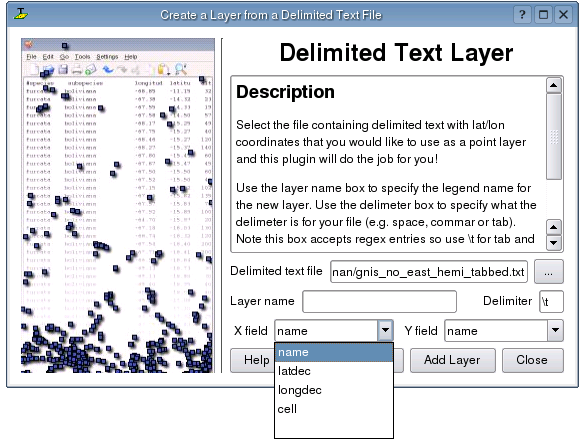
\includegraphics[clip=true, width=10cm]{file_selected2}
   \end{center}  
\end{figure}

Para analizar correctamente el archivo, cambie el delimitador a tabulador, 
usando \mbox{$\backslash$}t (esta es una expresión regular para el carácter 
tabulador). Después de cambiar el delimitador, pulse {\em Analizar}. Las 
casillas desplegables ahora contendrá los campos analizados correctamente como 
se muestra en la Figura \ref{fig:delim_text_file_selected2}.

\begin{figure}[ht]
   \begin{center}
   \caption{Seleccionar los campos X e Y}\label{fig:delim_text_file_selected3}\smallskip
\includegraphics[clip=true, width=10cm]{file_selected3}
   \end{center}  
\end{figure}

Seleccione los campos X e Y de los cuadros desplegables e introduzca un nombre 
de capa como se muestra en la Figura \ref{fig:delim_text_file_selected3}. Para 
añadir la capa al mapa pulse {\em Aceptar}. El archivo de texto delimitado ahora funcionará como cualquier otra capa de mapas en QGIS.

% html: End of file: `index.html'